Dla systemów agentowych kluczowym zagadnieniem jest stworzenie mechanizmów naprawczych. Należy założyć, że zarówno komunikacja pomiędzy agentami, jak i agenci jako procesy mogą ulec awarii. Sytuacje takie należy przede wszystkim wykryć oraz, jeśli jest to możliwe, naprawić. 

\subsection{Założenia}

Dla zaproponowanej przez nas architektury rozwiązania zdefiniowaliśmy wszystkie możliwe rodzaje awarii oraz ustaliliśmy z jakimi system będzie w stanie sobie poradzić. W rzeczywistości nie jest możliwe stworzenie mechanizmów uodparniających na wszystkie rodzaje awarii. 

W przypadku wykorzystania biblioteki \texttt{SPADE} zauważone zostało, że należy wyróżnić dwa rodzaje awarii:
\begin{enumerate}
	\item awarię pojedynczego zachowania agenta \texttt{FactoryAgent},
	\item awarię całego agenta \texttt{FactoryAgent},
	\item awarię pojedynczego zachowania agenta \texttt{ManagerAgent},
	\item awarię całego agenta \texttt{ManagerAgent}.
\end{enumerate}

Postanowiliśmy, że kluczowe z punktu widzenia algorytmu są agenty \texttt{FactoryAgent}. Z tego powodu nie zostały stworzone zachowania odpornościowe dla agenta zarządcy a sam \texttt{ManagerAgent} odgrywa istotną rolę w mechanizmach odpornościowych agentów \texttt{FactoryAgent}. 
 
Stworzono mechanizmy naprawcze dla następujących sytuacji:
\begin{itemize}
	\item wykrycie zabitego zachowania w \texttt{FactoryAgent}.
	\item brak odpowiedzi na wiadomości od współpracowników.
	\item brak odpowiedzi na wiadomość od \texttt{ManagerAgent}
\end{itemize}

Ponadto system pozwala na wykrycie awarii zachowania \texttt{ControlSubordinatesBehaviour}, czyli awarii \texttt{ManagerAgent}.

\subsection{Zaimplementowane mechanizmy}
Aby zrealizować mechanizmy odpornościowe zaprojektowano dwa zachowania: \texttt{ControlSubordinatesBehaviour} w \texttt{ManagerAgent} oraz \texttt{WatchdogBehaviour} w \texttt{FactoryAgent}.

Zadaniem \texttt{ControlSubordinatesBehaviour} jest monitorowanie działania poszczególnych agentów \texttt{FactoryAgent}. Jest to zachowanie cykliczne, które z określoną częstotliwością wysyła wiadomość typu \texttt{WatchdogMessage} do zachowań \texttt{WatchdogBehaviour} wszystkich podwładnych agentów. Zachowanie to oczekuje na odpowiedź z \texttt{WorkingState}. 

Enum \texttt{WorkingState} ma zdefiniowane trzy wartości: \texttt{OK}, \texttt{RESTARTING} oraz \texttt{COMPLAINT}. Pierwsze dwie wysyłane są do Managera w odpowiedzi na \texttt{WatchdogMessage}, a ostatnie wysyłane jest przez pozostałe zachowania agentów, jeśli nie będą one w stanie skontaktować się z współpracownikami. Diagram sekwencji dla mechanizmu naprawczego w momencie wykrycia nieodpowiadania na wiadomości przez współpracownika został przedstawiony na rysunku \ref{fig:recovery-kablowanie}.

Zachowanie \texttt{ControlSubordinatesBehaviour} zlicza ile razy pod rząd nie uzyskano odpowiedzi od poszczególnych podwładnych agentów lub uzyskano odpowiedź \texttt{RESTARTING}. Jeśli okaże się, że agenci nie odpowiadali lub próbowali zrestartować swoje zachowania ponad dwa razy pod rząd, manager restartuje agenta. Diagram sekwencji dla mechanizmu naprawczego agentów został przedstawiony na rysunku \ref{fig:recovery-pingowanie}.

Przy tworzeniu agenta w czasie trwania negocjacji istotne jest, aby przekazać mu dwie kluczowe zmienne stanu: jego aktywność oraz aktywność współpracowników. Są to zmienne krytyczne z punktu widzenia algorytmu negocjacji. 

Ponadto, jeśli restartowany agent aktywnie brał udział w negocjacjach, nie należy doprowadzić do desynchronizacji z pozostałymi agentami. Z tego powodu, we wszystkich synchronizowanych stanach dodano przejście do stanu \texttt{STATE\_PROPOSE}. 

Agenty, jeśli wykryją, że któryś z ich współpracowników zbyt długo nie przysłał wiadomości ze swoją informacją lub decyzją wysyłają do managera wiadomość ze skargą. W treści wiadomości zapisany jest jid agenta, który nie wysłał wiadomości. Zmiana stanu jest dokonywana, by ponownie zsynchronizować agenty. \texttt{STATE\_PROPOSE} jest pierwszym stanem wymagającym synchronizacji po dokonaniu inicjalizacji.

Zachowanie \texttt{WatchdogBehaviour} agenta \texttt{FactoryAgent} jest również cykliczne. Z zadaną częstotliwością sprawdza, czy przyszła wiadomość typu \texttt{WatchdogMessage} od zarządcy. Aby odpowiedzieć, sprawdza stan zachowań będącymi serwisami agenta oraz zwraca wartość \texttt{OK} jeśli wszystkie serwisy działają poprawnie lub \texttt{RESTARTING} jeśli okazało się, że któreś zachowanie został zabite. W sprawdzaniu zachowań pomięty został \texttt{NegotiateFSM}. Uznano, że restartowanie tego zachowania jest praktycznie równoznaczne z restartowaniem całego agenta. 

\begin{figure}[h]
	\centering
	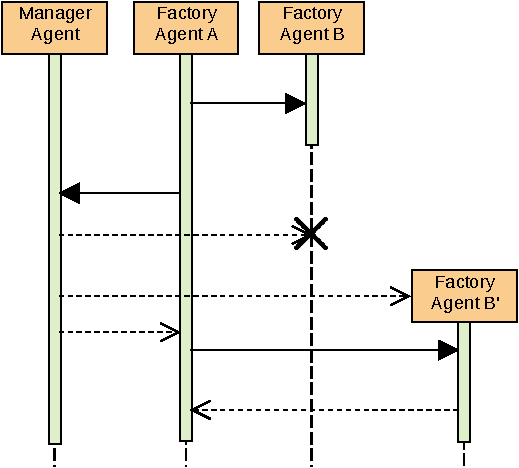
\includegraphics[width=0.8\columnwidth]{figures/SAG-Kablowanie.pdf}
	\caption{Diagram sekwencji dla mechanizmu naprawczego agentów w przypadku zgłaszania problemów z współpracownikiem}
	\label{fig:recovery-kablowanie}
\end{figure}

\begin{figure}[h]
	\centering
	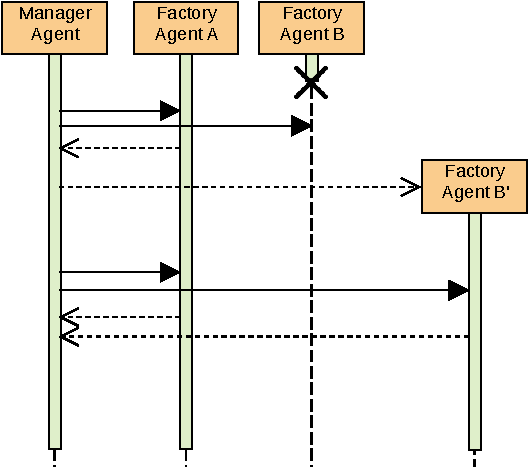
\includegraphics[width=0.8\columnwidth]{figures/SAG-Pingowanie.pdf}
	\caption{Diagram sekwencji dla mechanizmu naprawczego agentów w przypadku nieodpowiadania na zapytania \texttt{ManagerAgent}}
	\label{fig:recovery-pingowanie}
\end{figure}




